\documentclass[../main.tex]{subfiles}

\begin{document}

    A large portion of graph theory is concerned with the colouring of graphs such that no two adjacent vertices are coloured with the same colour. The Four Colour theorem \cite{gonthier2008formal} is one of the most celebrated theorem in the field of graph colouring, which provided the motivation for developing algebraic graph theory. It is also said to be the first theorem proved using significant help from computers. Graph colouring has many applications in computer science, information theory, and complexity theory, as well as many everyday problems, such as minimising conflicts in scheduling. 
    
    \begin{sloppypar}
    The accompanying notebook for this section can be found at \href{https://github.com/yangdabei/graph-colouring-and-sudoku/blob/main/example_graph_colouring.ipynb}{here}. Before we formulate a graph colouring problem to an ideal membership problem, we first give some key definitions.
    \end{sloppypar}

    \begin{definition}
        A \emph{graph} is an ordered pair $G=(V,E)$, which consists of a nonempty set $V$ of \emph{vertices} and a set $E$ of paired vertices whose elements are called \emph{edges}.
    \end{definition}
    For this report, we only consider \emph{simple graphs}, that is, graphs that do not have more than one edge between two vertices and no edges that start and end at the same vertex. 
    \begin{definition}
        Let $G=(V,E)$ be an $n$-vertex graph. For a vertex $v\in V$, the \emph{neighbourhood} of $v$ is given by $N(v)=\{u\in V\, |\, \{u,v\}\in E\}$. 
    \end{definition}
    \begin{definition}
        Let $G=(V,E)$ be a graph containing an edge $e = \{u,v\}$ with $u\neq v$. Let $f$ be a function that is the identity on $V\setminus \{u,v\}$ and sends $u$ and $v$ to $w$. The \emph{edge contraction} of $e$, denoted by $G/e$, results in a new graph $G'=(V', E')$ where $V'=V\setminus \{u,v\} \cup \{w\}$ and $E'=E\setminus \{e\}$. The \emph{deletion} of $e$, denoted by $G-e$, is the graph $G'=(V,E\setminus \{e\})$.
    \end{definition}
    Put simply, the edge contraction of $e=\{u,v\}$ removes the $e$ and merges the two vertices $u$ and $v$, and edge deletion removes an edge between two vertices.
    \begin{definition}
        For a graph $G=(V,E)$, a \emph{colouring} is a function $\mathcal{C}:V\to \{1,2,\dots\}$ such that for all $u\in N(v)$, $\mathcal{C}(u)\neq\mathcal{C}(v)$. $G$ is $k$-colourable if $G$ can be coloured with $k$ distinct colours. A subset of vertices with the same colour forms a \emph{colour class}.
    \end{definition}

    We now ask the question, given a graph, is it $k$-colourable?

    \subsection{Determining $k$-colourability}
    \subsubsection{Quotient Method}

    We introduce a tool that helps us transform a graph colouring problem into a set of polynomial equations that we can solve. The theorem after gives the relation between the decidability of a $k$-colouring of a graph and ideal membership.

    \begin{definition} \label{def:graph polynomial}
        The \emph{graph polynomial} $f_G$ associated to the graph $G=(V,E)$ is an element of the ring $\mathbb{C}[x_1,\dots,x_n]$, given by:
        $$f_G := \prod_{\{u,v\}\in E}(u-v)$$
    \end{definition}

    \begin{theorem}
        Fix $k$ a positive integer. Let $I$ be the ideal generated by the polynomials $x^k-1$ for $x\in V$. The graph $G$ is $k$-colourable if and only if $f_G\notin I$.
        \begin{proof}
            Let $G$ be $k$-colourable. Then there is an assignment of colours to the vertices such that no two adjacent vertices have the same colour. This corresponds to a point $a\in \mathbf{V}(I)$ such that $f_G(a)\neq 0$. Hence, $f_G\notin I$.

            Conversely, if $G$ is not $k$-colourable, then there is at elast one pair of adjacent vertices that share a colour. This means that $f_G$ vanishes for any assignment of colours, that is, $f_G$ vanishes on $\mathbf{V}(I)$. By Hilbert's Nullstellensatz, there is some $m$ such that $f_G^m\in I$. This implies that $f_G^m(a)=0$ for $a\in \mathbf{V}(I)$. Because $\mathbb{C}$ is a field, $f_G^m(a)=0$ implies that $f_G(a)=0$. Hence, $f_G\in I$.
        \end{proof}
    \end{theorem}

    One can view the above theorem in this way: for each $v\in V$, the polynomials that generate $I$ represent the $k$-th roots of unity. We assign a colour to each vertex, where each colour corresponds to a $k$-th root of unity. Then, if two adjacent vertices are assigned the same colour, $f_G$ will vanish. This criterion allows us to perform an algorithm to determine if a graph is $k$-colourable: compute a Gr\"obner basis for $I$, and then divide $f_G$ by this basis.

    \subsubsection{Roots of Unity Method} \label{subsec:roi}
    
    We can also generate the ideal in a way such that we can check whether there is a solution in the variety corresponding to the ideal. Let $x=e^{\frac{2\pi i}{k}}\in \mathbb{C}$ be the $k$-th root of unity. Represent the $k$ colours by the $k$ distinct roots of unity, so each vertex is assigned $1, x, x^2,\dots,x^{k-1}$. For $1\leq i\leq n$, we can model this as
    \begin{equation} \label{eq:k_roots}
        x_i^k-1=0.
    \end{equation}
    Now, if $x_i$ and $x_j$ are connected by an edge, they need to be a different colour. Since $x_i^k = x_j^k$, we have that $(x_i-x_j)(x_i^{k-1} + x_i^{k-2}x_j+\dots+x_ix_j^{k-2}+x_j^{k-1})$. We require $x_i$ and $x_j$ to be different $k$-th roots of unity so 
    \begin{equation} \label{eq:edges}
        x_i^{k-1} + x_i^{k-2}x_j+\dots+x_ix_j^{k-2}+x_j^{k-1}=0.
    \end{equation}
    Let the ideal $I$ be generated by the polynomials in Equation \ref{eq:k_roots} as well as by the polynomials in Equation \ref{eq:edges} for each pair of adjacent vertices $x_i, x_j$ . We call this system of polynomial equations the \emph{roots of unity} system.
    \begin{definition}
        The $k$-colouring of an $n$-vertex graph $G$ given by the \emph{roots of unity system} is the ideal $I\subseteq \mathbb{C}[x_1,\dots,x_n]$ generated by 
        \begin{align*}
            \text{for all $i\in V(G)$}&: \quad x_i^k-1 \\
            \text{for all $\{i,j\}\in E(G)$}&: \quad x_i^{k-1} + x_i^{k-2}x_j+\dots+x_ix_j^{k-2}+x_j^{k-1}
        \end{align*}
    \end{definition}

    Since $\mathbf{V}(I) = \emptyset$ implies that $I=\mathbb{C}[x_1,\dots,x_n]$ by the Weak Nullstellensatz, we can check whether $1\in I$. If this is true, then there are no solutions to the graph colouring problem. 

    \begin{figure} [H]
        \centering
        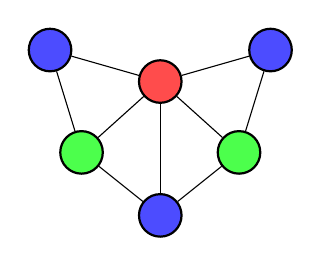
\begin{tikzpicture}
            [rednode/.style={scale=.9, auto=center, circle, draw=black, fill=red!70, thick, minimum size=6mm},
            green/.style={scale=.9, auto=center, circle, draw=black, fill=green!70, thick, minimum size=6mm},
            blue/.style={scale=.9, auto=center, circle, draw=black, fill=blue!70, thick, minimum size=6mm}]

            \node[blue] (a1) at (0,0) {};
            \node[green] (a2) at (-1,0.8) {};
            \node[green] (a3) at (1,0.8) {};
            \node[rednode] (a4) at (0,1.7) {};
            \node[blue] (a5) at (-1.4, 2.1) {};
            \node[blue] (a6) at (1.4,2.1) {};

            \draw (a1) -- (a2);
            \draw (a1) -- (a3);
            \draw (a1) -- (a4);
            \draw (a2) -- (a4);
            \draw (a3) -- (a4);
            \draw (a4) -- (a5);
            \draw (a4) -- (a6);
            \draw (a2) -- (a5);
            \draw (a3) -- (a6);
                    

        \end{tikzpicture}
        \caption{A graph colouring for a graph with six vertices. It can be coloured with three colours so it is 3-colourable. However, it cannot be coloured with two colours, so it has chromatic number $\chi(G)=3$.}
 
        \label{fig:chromatic colour}
    \end{figure}



    \subsection{The Chromatic Number}

    Another interesting question that arises from the colouring problem is what the smallest number of colours required to colour a graph. The accompanying notebook to this subsection can be found \href{https://github.com/yangdabei/graph-colouring-and-sudoku/blob/main/example_chromatic_number.ipynb}{here}. We first give the following definition.

    \begin{definition}
        The \emph{chromatic number} $\chi=\chi(G)$ is the smallest number such that the graph can be coloured with $\chi$ colours. A $k$-colourable graph is $k$-chromatic if its chromatic number is $k$.
    \end{definition}
    Figure \ref{fig:chromatic colour} gives the chromatic number for an example graph. We will now discuss the covering ideal of a graph and its connection to its chromatic number.

    \begin{definition}
        For a graph $G=(V,E)$, an \emph{independent set} is a set of vertices $U\subseteq V$ such that there are no edges between any two vertices in $U$. The independence number is the size of the largest independent set. A subset $W\subseteq V$ is a \emph{vertex cover} such that for all $\{u,v\}\in E$, $u\in W$ or $v\in W$. 
    \end{definition}

    It follows that a vertex cover of a graph is the complement of an independent set. Hence, a maximal independent set corresponds to a minimal vertex cover. Furthermore, each vertex in an independent set can be coloured the same colour. Therefore, from definitions, we get the following lemma.

    \begin{lemma} \label{lem:independent vertex cover}
        Let $G=(V,E)$ be a graph and $U\subseteq V$ be a subset of vertices. Then $U$ is an independent set if and only if $V\setminus U$ is a vertex cover.
    \end{lemma}

    \begin{definition}
        For a graph $G$, the \emph{cover ideal} $I_{cover}(G)$ is the monomial ideal
        $$I_{cover}(G) := \bigcap_{\{u,v\}\in E}\langle u,v\rangle$$
    \end{definition}
    We will see that the minimal generators for $I_{cover}(G)$ will correspond to minimal vertex covers for $G$. Since the minimal vertex cover is the complement of a maximal independent set, then $I_{cover}(G)$ will be related to the independence number of $G$.

    \begin{proposition} \label{prop:minimal vertex cover}
        Let $G$ be a graph and $W\subseteq V$ a minimal vertex cover. Let $J$ be the cover ideal of $G$. Then $J$ is generated by monomials of the form $\prod_{w\in W} w$.
    \end{proposition}
    \begin{proof}
        Let $x_W$ denote the product of variables for any $W\subseteq V$, and let $I$ be the ideal generated by \{$x_{W_{min}}\}$, where $W_{min}$ is a minimal vetex cover. Suppose that $W$ is a minimal vetex cover. Then for any edge $\{u,v\}\in E$, either $u\in W$ or $v\in W$. This means that either $u$ divides $x_W$ or $v$ divides $x_W$, and so, $x_W\in \langle u,v\rangle$. Hence, $x_W\in J$, so $I\subseteq J$. Conversely, let $f\in J$ be any monomial generator and let $W$ be the set of variables which can divide $f$. Since $f\in J$, then $f\in \langle u,v\rangle$ for each edge $\{u,v\}\in E$. This means that either $u$ divides $f$ or $v$ divides $f$, so either $u\in W$ or $v\in W$. Hence, $W$ is a vertex cover. Let $W'\subseteq W$ be a minimal vertex cover. Since $x_{W'}$ divides $f$, $f\in I$. Hence, $J\subseteq I$.
    \end{proof}

    We have already established that minimal vertex covers are the compliments of maximal independent sets, so the generators of $I_{cover}(G)$ also correspond to the maximal independent sets of $G$. Using this fact, we prove the following theorem from \cite{francisco2011colorings}.

    \begin{theorem} \label{thm:chromatic number}
        Let $G$ be a graph a vertex set $V=\{x_1,\dots,x_n\}$ with cover ideal $J$. Then $x_V^{d-1}\in J^d$ if and only if $\chi(G)\leq d$, where $x_V=x_1\dots x_n$. In particular,
        $$\chi(G)=\min\{d\,|\,x_V^{d-1}\in J^d\}.$$
    \end{theorem}
    \begin{proof}
        First, let $U_1\cup\dots\cup C_{\chi(G)}$ be a $\chi(G)$-colouring of $G$, where each $U_i$ contains vertices in the same colour class. It is also an independent set. By Lemma \ref{lem:independent vertex cover}, we have that for each $i=1,\dots,\chi(G)$, 
        $$W_i=U_1\cup\dots \cup U_{i-1} \cup U_{i+1}\cup\dots\cup U_{\chi(G)}$$
        is a vertex cover of $G$. Hence, $x_{W_i}\in J$ for $i=1,\dots, \chi(G)$. It follows that 
        $$\prod^{\chi(G)}_{i=1}x_{W_i}= \lr(){\prod^{\chi(G)}_{i=1}x_{U_i}}^{\chi(G)-1}=(x_1\dots x_n)^{\chi(G)-1}=x_V^{\chi(G)-1}\in J^{\chi(G)}.$$
        The first equality comes from the fact that the colour classes $U_i$ are disjoint so if a vertex $x_i\in U_j$, then $x_i\in W_k$ for all $k\neq j$. Hence each vertex appears $\chi(G)-1$ times in $x_{W_1}\dots x_{W_{\chi(G)}}$. Hence, $x_V^{d-1} =x_V^{\chi(G)-1}x_V^{d-\chi(G)}\in J^{\chi(G)}\cdot J^{d-\chi(G)} = J^d$ since $x_V\in J$.

        Conversely, suppose that $x_V^{d-1}\in J^d$. Then there exists $d$ minimal vertex covers $W_1,\dots, W_d$, which are not necessarily disinct, such that $x_{W_1}\dots x_{W_d}$ can divide $x_V^{d-1}$. Using a similar argument from above, this is because for each $x_i\in \{x_1,\dots,x_n\}$, there exists some $W_j$ such that $x_i\notin W_j$, since if $x_i\in W_j$ for all $1\leq j\leq d$, the power of $x_i$ is $d$ in $x_{W_1}\dots x_{W_d}$. This gives a contradiction since it cannot divide $x_V^{d-1}$. Now, we want to form complements of $W_i$ in a way that gives a $d$-colouring of $G$. Form the following $d$ sets as follows:
        \begin{align*}
            U_1 &= V\setminus W_1 \\
            U_2 &= (V\setminus W_2) \setminus U_1 \\
            U_3 &= (V\setminus W_3) \setminus (U_1\cup U_2) \\
            &\vdots \\
            U_d &= (V\setminus W_d) \setminus (U_1\cup\dots \cup U_{d-1}).
        \end{align*}
        It suffices to show that $U_1,\dots , U_d$ form a $d$-colouring of $G$. First, note that each $U_i$'s are disjoint by construction. Also, because each $U_i\subseteq V\setminus W_i$, each $U_i$ is an independent set. Then it remains to show that $V=U_1\cup\dots\cup U_d$. If we have $x\in V$, then there exists some $W_j$ such that $x\notin W_j$, so $x\in V\setminus W_j$. Hence, either $x\in U_j$ or $x\in (U_1\cup\dots\cup U_{j-1})$ for $j\leq d$.

        




        %First, let $\chi(G)=d$. We then partition $V$ into its colour classes such that %$V=U_1\cup \dots\cup U_d$. Since each $U_i$ is an independent set of $G$, let %$W_i=V\setminus U_i$ be the corresponding vertex colouring. By Proposition \ref%{prop:minimal vertex cover}, we have that $x_{W_i}\in I_{cover}(G)$. If we multiply %these monomials together, we have that $x_{W_1}\dots x_{W_d}\in J^d$. However, %since all the $U_i$'s are disjoint, if $x_i\in U_j$, then $x_i\in W_k$ for $k\neq %j$. Hence, each vertex appears $d-1$ times in $x_{W_1}\dots x_{W_d}$. Therefore, $x_%{W_1}\dots x_{W_d}=x_V^{d-1}\in J^d$. Conversely, let $x_V^{d-1}\in J^d$. Then, %there exists $d$ minimal vertex covers $W_1,\dots,W_d$ (not necessarily distinct) %such that $x_{W_1}\dots x_{W_d} | x_V^{d-1}$. For each $x_i\in \{x_1,\dots,x_n\}$, %there exists 
    \end{proof}

    \begin{example}
        Consider the graph $G=C_5$, which is the cyclic graph with five nodes. The vertices coloured in blue form an independent set since they share no edges. The uncoloured vertices form a vertex cover since any edge has an endpoint among the uncoloured vertices.
        
        \begin{figure}[H]
            \centering
            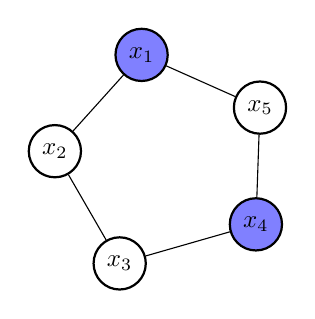
\begin{tikzpicture}
                [rednode/.style={scale=.9, auto=center, circle, draw=black, fill=red!70, thick, minimum size=6mm},
                green/.style={scale=.9, auto=center, circle, draw=black, fill=green!70, thick, minimum size=6mm},
                blue/.style={scale=.9, auto=center, circle, draw=black, fill=blue!50, thick, minimum size=6mm},
                roundnode/.style={scale=.9, auto=center,circle, draw=black, fill=white, thick, minimum size=6mm},]

                \node[blue] (a1) at ({72*1+30}:1.4) {$x_1$};
                \node[roundnode] (a2) at ({72*2+30}:1.4) {$x_2$};
                \node[roundnode] (a3) at ({72*3+30}:1.4) {$x_3$};
                \node[blue] (a4) at ({74*4+30}:1.4) {$x_4$};
                \node[roundnode] (a5) at ({72*0+30}:1.4) {$x_5$};

                \draw (a1) -- (a2);
                \draw (a2) -- (a3);
                \draw (a3) -- (a4);
                \draw (a4) -- (a5);
                \draw (a5) -- (a1);
  
                
            \end{tikzpicture}
        \end{figure}

        Let $J$ be the cover ideal for this graph. Apply Proposition \ref{prop:minimal vertex cover} and we have that $J = \langle x_1,x_2\rangle \cap \langle x_2,x_3\rangle \cap \langle x_3,x_4\rangle \cap \langle x_4,x_5\rangle \cap \langle x_5,x_1\rangle$. Using a computer algebra simplifier, we have that $$J = \langle x_2x_4x_5, x_2x_3x_5, x_1x_3x_5, x_1x_3x_4,x_1x_2x_4\rangle,$$
        which corresponds to the minimal vertex covers of $G$.

        By inspection, we see that $\chi(G)=3$. However, we wish to confirm Theorem \ref{thm:chromatic number}. What is the minimal $d$ such that $(x_1x_2x_3x_4x_5)^{d-1}\in J^d$? For $d=1$, we have that $1\notin J$, so $G$ is not 1-colourable. For $d=2$, $J^2$ is generated by pairwise products of the generators of $J$, so $J^2$ is generated by monomials of degree 6. Hence, $x_1x_2x_3x_4x_5\notin J^2$. Finally, for $d=3$, $J^3$ is generated by products of any three of the monomial generators of $J$. We find that $x_1x_2^2x_3^2x_4^2x_5^2=(x_2x_4x_5)\cdot(x_2x_3x_5)\cdot(x_1x_3x_4)$. Hence, $x_1\cdot x_1x_2^2x_3^2x_4^2x_5^2 = x_1^2x_2^2x_3^2x_4^2x_5^2\in J^3$ so the $\chi(G)=3$.
    \end{example}

    

    \subsection{Chromatic Polynomials}

    As an aside, we explore the $k$-colourability of a graph by introducing the chromatic polynomial which is a key object in the study of algebraic graph theory. This section describes the problem in a more graph theoretic manner. 

    \begin{theorem}
        The chromatic function of a graph $G=(V,E)$ is a polynomial.
    \end{theorem}
    \begin{proof}
        Before our discussion on chromatic polynomials, we want to show that they are indeed polynomials. Construct colourings of $G$ by partitioning $V$ into independent sets and assigning a unique to colour to each independent set. Given $k$ colours, there are $k$ ways to choose a colour for the first set, $(k-1)$ ways for the second, and so on. Hence, there are $k(k-1)(k-2)\dots$ possible ways to colour a graph $G$ such that it results in a proper colouring. This is a polynomial in $k$.
    \end{proof}

    \begin{definition}
        The \emph{chromatic polynomial} $P(G,x)$ for a graph $G$ is a unique polynomial, which evaluated at any integer $k\geq0$ coincides with $P(G,k)$, the number of $G$'s proper $k$-colourings.
    \end{definition}
    \begin{theorem}
        Let $G$ be an $n$-vertex graph. Let $C$ be a partial proper colouring of $c$ vertices of $G$ using $d_0$ colours. Let $P(G_C,k)$ be the number of ways of completing this colouring using $k$ colours to obtain a proper colouring of $G$. Then $P(G_C,k)$ is a monic polynomial in $k$ with integer coefficients of degree $n-c$ for $k\geq d_0$.
    \end{theorem}
    \begin{proof}
        We prove the above theorem using induction on the number of edges of the graph $G$ with a partial colouring $C$. Consider the three cases:
        \begin{enumerate}
            \item[Case 1.] Suppose that $\{u,v\}$ is an edge connecting vertices $u$ and $v$ of $G$ where at most one of which is contained in $C$. Now, each proper colouring of $G$ is also a proper colouring of $G-e$ since the deletion of the edge has no effect on an already coloured graph. Each proper colouring of $G-e$ is also a proper colouring of $G$ if and only if the endpoints of $e$ are distinct vertices $u$ and $v$. Hence, the number of proper colourings $P(G_C, k)$ can be obtained from $P(G_C-e,k)$ by subtracting the colourings that assigns the same colour to $u$ and $v$ which is given by $P(G_C/e,k)$. We get that
            $$P(G_C,k) = P(G_C-e,k)-P(G_C/e, k).$$
            (This can also be shown from the deletion-contraction recurrence formula or \textbf{Fundamental Reduction Theorem} \cite{dong2005chromatic}). Since $G-e$ and $G/e$ have fewer edges than $G$, we can apply induction to complete the proof in this case.

            \item[Case 2.] Suppose that $G$ has one vertex $v_0$ not contained in $C$. If this vertex is not adjacent to any vertex of $G$, then $G=C\cup \{v_0\}$, which is a disjoint union. Hence, we can colour $v_0$ any of the $k$ colours. If this vertex is adjacent to $d$ vertices of $C$ which use $d_0$ colours, then $P(G_C,k)=\max\{k-d_0,0\}$.
            
            \item[Case 3.] Suppose that ever vertex of $G$ is contained in $C$. Then, we already have a colouring of $G$ and $P(G_C,k)=1$.
        \end{enumerate}
        Hence, by induction the number of edges, the theorem is proved.
    \end{proof}

    \begin{figure}[!h] 
        \centering
        
        \begin{subfigure}[b]{0.3\textwidth}
            \centering
            \subcaptionbox{Partial colouring of $G$. If $x_2$ is green, $x_3$ must be blue and $x_4$ can be either red or green, so we get two 3-colourings. We get two more if we set $x_2$ to be blue, give a total of four 3-colourings}[1\linewidth]{
                \begin{tikzpicture}  
                    %[scale=.9,auto=center,every node/.style={circle,fill=blue!20}] %  
                    [
                        rednode/.style={scale=.9, auto=center, circle, draw=black, fill=red!70, thick, minimum size=6mm},
                        roundnode/.style={scale=.9, auto=center,circle, draw=black, fill=white, thick, minimum size=6mm},
                    ]
                    
                    \node[rednode] (a1) at (1,2.3) {$x_1$};  
                    %\node[roundnode] (a2) at (-0.25,4)  {$x_2$};
                    \node[semifill={upper=blue!20, lower = green!20, ang = -45}] (a2) at (-0.25,4)  {$x_2$}; 
                    \node[semifill={upper=green!20, lower = blue!20, ang = -45}] (a3) at (2.25,4)  {$x_3$}; 
                    %\node[roundnode] (a3) at (2.25,4)  {$x_3$}; 
                    %\node[semifill={upper=red, lower = green, ang = -45}] (a4) at (4.2,4) {$x_4$};  
                    \node[roundnode] (a4) at (4.2,4) {$x_4$};  
                    
                    
                    \draw (a1) -- (a2); % these are the straight lines from one vertex to another  
                    \draw (a2) -- (a3);  
                    \draw (a3) -- (a1);  
                    \draw (a3) -- (a4); 
                    
                \end{tikzpicture}  
            }
    \end{subfigure}
    \hfill
    \begin{subfigure}[b]{0.3\textwidth}
        \centering
        
        \subcaptionbox{$G-\{x_2,x_3\}$. Now, $x_2$ and $x_3$ can be the same colour. There are two options for $x_2$, $x_3$, and $x_4$, giving eight 3-colourings.}[1\linewidth]{
            \begin{tikzpicture}  
            %[scale=.9,auto=center,every node/.style={circle,fill=blue!20}] % 
            [
                rednode/.style={scale=.9, auto=center, circle, draw=black, fill=red, thick, minimum size=6mm},
                roundnode/.style={scale=.9, auto=center,circle, draw=black, fill=white, thick, minimum size=6mm},
            ]
              
            \node[rednode] (a1) at (1,2.3) {$x_1$};  
            %\node[roundnode] (a2) at (-0.25,4)  {$x_2$}; 
            %\node[roundnode] (a3) at (2.25,4)  {$x_3$}; 
            \node[semifill={upper=blue!20, lower = green!20, ang = -45}] (a2) at (-0.25,4)  {$x_2$}; 
            \node[semifill={upper=blue!20, lower = green!20, ang = -45}] (a3) at (2.25,4)  {$x_3$};  
            \node[roundnode] (a4) at (4.2,4) {$x_4$};  
            
            
            \draw (a1) -- (a2); 
            %\draw (a2) -- (a3);  
            \draw (a3) -- (a1);  
            \draw (a3) -- (a4); 
            
        \end{tikzpicture}  
        }
    \end{subfigure}
    \hfill
    \begin{subfigure}[b]{0.3\textwidth}
        \centering
        
        \subcaptionbox{$G/\{x_2,x_3\}$. The vertices $x_2$ and $x_3$ has been replaced by $w$. There are two ways of colouring $w$ and two ways of colouring $x_4$, giving four 3-colourings.}[1\linewidth]{
            \begin{tikzpicture}  
                %[scale=.9,auto=center,every node/.style={circle,fill=blue!20}] 
                [
                    rednode/.style={scale=.9, auto=center, circle, draw=black, fill=red, thick, minimum size=6mm},
                    roundnode/.style={scale=.9, auto=center,circle, draw=black, fill=white, thick, minimum size=6mm},
                ]
                  
                \node[rednode] (a1) at (2.25,2.3) {$x_1$};  
                %\node (a2) at (-0.25,4)  {2}; %
                \node[semifill={upper=blue!20, lower = green!20, ang = -45}] (a3) at (2.25,4)  {$w$};  
                \node[roundnode] (a4) at (4.2,4) {$x_4$};  
                
                
                %\draw (a1) -- (a2); 
                %\draw (a2) -- (a3);  
                \draw (a3) -- (a1);  
                \draw (a3) -- (a4); 
                
            \end{tikzpicture}  
        }
    \end{subfigure}
    \caption{3-colourings of a graph $G$ given a partial colouring with deletion and contraction.}
    \label{fig:deletion contraction}
    \end{figure}

    Case 1 in the above proof uses the deletion-contraction formula. We see an example in Figure \ref{fig:deletion contraction} where $P(G_C,3)=P(G_C-\{x_2,x_3\},3)-P(G_C/\{x_2,x_3\},3) = 8-4 = 4$. Next, it would be very interesting to understand the conditions under which a partial colouring can be extended to a unique colouring. This motivates the following result.

    \begin{theorem} \label{th:partial}
        Let $G$ be a graph with chromatic number $\chi(G)$ and $C$ be a partial colouring of $G$ using $\chi(G)-2$ colours. Then there are at least two ways of extending the colouring if the partial colouring can be completed to a total proper colouring of $G$.
    \end{theorem}
    \begin{proof}
        If the partial colouring only uses $\chi(G)-2$ colours, then the two colours left can be used interchangeably to complete the partial solution to a total proper colouring. Hence, there are at least two ways of extending to a full solution by swapping the two colours used.
    \end{proof}
    Theorem \ref{th:partial} implies that there exists a unique solution for a partial colouring $C$ if $C$ uses at least $\chi(G)-1$ colours. We introduce Sudoku puzzles in the next section, but it is insightful to know that for any $9\times 9$ Sudoku puzzle, at least eight numbers must be used in the clues \cite{herzberg2007sudoku}. In general, for an $n^2\times n^2$ Sudoku puzzle, at least $n^2-1$ numbers must be used in a given partial solution for it to have a unique solution.

\end{document}